The photons selected for use in this analysis are initially taken from the PF photon candidates described in Sec.~\ref{sec:evt_pf}.
In further reconstruction of photons for \Hgg analyses, there are several challenges to overcome.
First, the energy estimate provided by the PF algorithm generally has inherent bias.
The bias in the photon energy estimates are corrected for with a regression technique which utilizes \Zee events in which the electrons have been reconstructed as photons.
The procedure, described in Sec.~\ref{sec:evt_photon_energy} exploits the fact that the mass of the Z boson is known FIXME:CITE to good precision, ensuring that the \mee distribution is centered around \mZ.
An additional smearing procedure corrects for the differences in energy resolution between data and simulation.
This step is vital as simulation, not data, is used to construct the models of SM Higgs boson production modes, including \ttH.
A second challenge in \Hgg analyses is distinguishing between ``prompt'' photons and ``fake'' photons.
Prompt photons are those produced in the decay of the Higgs boson or from the primary hard inelastic scattering process (FIXME:feynman) and are typically the objects of interest of physics analyses.
Fake photons are those produced in hadronic jets, usually through the decay \Pigg (FIXME:feynman), and are (typically) of less interest.
Prompt photons tend to be more isolated in the detector and tend to have different shower shapes in the ECAL.
These differences are exploited through the used of a BDT trained to distinguish between prompt and fake photons.
The photon ID BDT, described in Sec.~\ref{sec:evt_photon_idmva}, uses a variety of high-level variables describing the photon's kinematics, shower shape, and isolation.
The shower shape \& isolation variables and the photon ID BDT are used to select photons of interest for the \ttH analysis, rejecting as many fake photons as possible while retaining a high efficiency on prompt photons.
As simulation is used to construct the models of SM Higgs boson production modes, it is important that the shower shape \& isolation variables and the photon ID BDT are well-described in simulation.
A chained quantile regression method, described in Sec.~\ref{sec:evt_photon_ss}, corrects the distributions of these features in simulation.
The multitude of high-level variables used to describe photons are defined in Sec~\ref{sec:evt_photon_vardef}.
 
\subsection{Variable Definitions} \label{sec:evt_photon_vardef}
The variables defined in this section are used for studying the scale \& resolution of photon energy reconstruction, discriminating between prompt and fake photons, selecting the photons to be used in analysis, or a combination of the three.

\subsubsection*{General}
\begin{itemize}
    \item \emph{Conversion-safe electron veto}: a flag rejecting the photon candidate if there is a track with at least one hit in the inner layer of the pixel detector pointing to the photon supercluster \emph{and} the track is not matched to a vertex. 
    \item \emph{Pixel seed veto}: a flag rejecting the photon candidate if any track with at least two hits points to the photon supercluster. In general, the pixel seed veto provides a more severe rejection of electrons but excludes a larger fraction of photons.
    \item $\rho$: the median energy density per unit area in the event. 
\end{itemize}

The pixel seed veto is, in general, much stricter than the conversion-safe electron veto in rejecting electrons imitating photons.
For most \Hgg analyses, electrons are not a large source of fake photons and so the conversion-safe electron veto is used for its greater efficiency on real photons.
However, the \ttH analysis has a significant background component coming from \ttplusX events in which an electron from a $\PW \to \Pe\nu_{\Pe}$ decay is reconstructed as a photon.
To target this background, the pixel seed veto is employed (as a training variable in the BDT used to define signal regions).

\subsubsection*{Shower shape variables}
\begin{itemize}
    \item $E_{2\times2}/E_{5\times5}$: the ratio of energies between $2\times2$ and $5\times5$ matrices of ECAL crystals. The $2\times2$ matrix is defined as that containing the two most energetic crystals, the $5\times5$ matrix is defined as that centered on the supercluster seed crystal.
    \item \emph{cov}$_{i\eta i\phi}$: the covariance of the crystal values of the $5\times5$ matrix centered on the supercluster seed crystal.
    \item $\sigma_{i\eta i\eta}$: the standard deviation along the $\eta$ direction of the electromagnetic shower (expressed in terms of crystal cells).
    \item $R_9$: $E_{3\times3}/E_{\text{SC}}$, where $E_{3\times3}$ is the $3\times3$ crystal matrix centered on the supercluster seed crystal and $E_{\text{SC}}$ is the total energy of the supercluster.
    \item $\sigma_\eta$: the standard deviation of crystal $\eta$ values in the supercluster, with each crystal's contribution weighted by the logarithm of its energy.
    \item $\sigma_\phi$: the standard deviation of crystal $\phi$ values in the supercluster, with each crystal's contribution weighted by the logarithm of its energy.
    \item \emph{Preshower} $\sigma_{RR}$: the standard deviation of the shower spread in the $x$ and $y$ directions of the preshower detector (defined only in the endcap).
\end{itemize}

The shower shape variables are useful in both the regression of photon energy and the discrimination between prompt photons and hadronic jets misidentified as photons (``fake'' photons).

\subsubsection*{Isolation variables}
\begin{itemize}
    \item $\mathcal I_{\text{ph}}$: the transverse energy sum of all other PF photons in a cone size $R=0.3$ around the photon candidate.
    \item $\mathcal I_{\text{ch, sel}}$: the transverse energy sum of all PF charged hadrons in a cone size $R=0.3$ around the photon candidate, measured with respect to the selected vertex.
    \item $\mathcal I_{\text{ch, wst}}$: the transverse energy sum of all PF charged hadrons in a cone size $R=0.3$ around the photon candidate, measured with respect to the worst-fit vertex.
    \item $H/E$: the energy sum from the HCAL towers within a cone of $R=0.15$ around the supercluster, divided by the energy of the supercluster.
    \item $\mathcal I_{\text{tk}}$: the transverse momentum sum of all tracks in a cone size $R=0.3$ around the photon candidate. Tracks within an inner cone size $R=0.04$ are \emph{not} included in this sum, effectively making the sum over a ``hollow'' cone.
\end{itemize}

The isolation variables are useful in discriminating between prompt photons and hadronic jets misidentified as photons.

\subsection{Energy Scale \& Resolution Corrections} \label{sec:evt_photon_energy}
The energy measurements of individual ECAL channels are first corrected, as described in Sec.~\ref{sec:cms_ecal}.
Once the ECAL energy measurements are calibrated, a multivariate regression technique~\cite{Khachatryan:2015iwa} is used to further correct the energy of photon candidates.
After the multivariate regression is applied, further energy scaling is applied to correct for any time or position dependent bias effects in the energy measurements in data.
Lastly, a smearing procedure is applied to simulation such that the energy resolution from simulation matches that in data.

The multivariate regression attempts to correct for many systematic sources of bias in the supercluster energy measurement.
For example, the supercluster may not capture all of the electromagnetic shower from a given photon (thereby underestimating its energy).
These sources typically relate to the details of the ECAL geometry (i.e. the geometrical arrangement of crystals and voids between crystals) and the probability of interaction with detector material before reaching the ECAL.
Among the training inputs for the regressor are the supercluster coordinates ($\eta$ and $\phi$), shower shape variables, information about the seed crystal of the supercluster, and variables ($\rho$ and number of vertices) describing the pileup conditions of the event. 

The regressor attempts to predict the form of the probability distribution function for $E_{\text{true}}/E_{\text{raw}}$.
The functional form for the probability distribution function for $E_{\text{true}}/E_{\text{raw}}$ is chosen as a Gaussian with two power law tails.
The regressor simultaneously predicts the true energy and the uncertainty in the energy measurement for a given photon, by returning values of the parameters for the functional form.
The true energy, $E_{\text{true}}$ is taken as the most probable value of the probability distribution function returned by the regressor.
The energy resolution is determined from the width of the probability distribution function. 
The sum of probability distribution functions returned by the regressor are compared to the actual $E_{\text{true}}/E_{\text{raw}}$ distribution (in simulation) in Fig.~\ref{fig:photon_energy_regression}.
\begin{figure} [h!]
    \centering 
    \begin{tabular}{c c}
        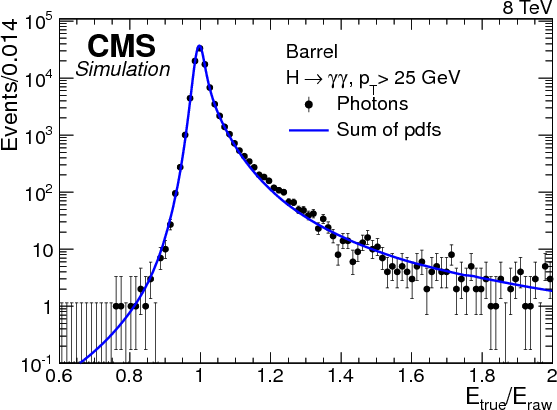
\includegraphics[width=0.48\linewidth]{figures/event_reconstruction_and_selection/figs_recoenergy_Fig-2a.png} &
        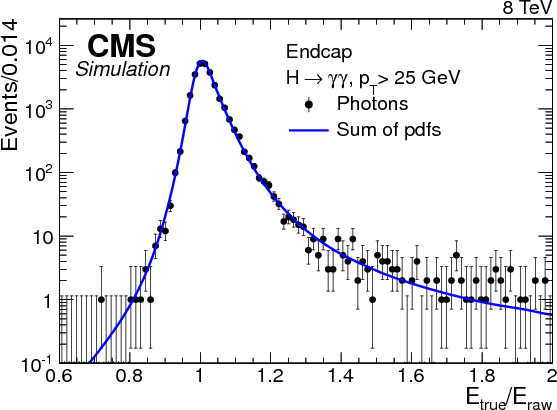
\includegraphics[width=0.48\linewidth]{figures/event_reconstruction_and_selection/figs_recoenergy_Fig-2b.png}
    \end{tabular}
    \caption{Sum of probability distribution functions returned by the regressor (blue) compared with the actual $E_{\text{true}}/E_{\text{raw}}$ distribution in simulation (black). Taken from~\cite{Khachatryan:2015iwa}}
    \label{fig:photon_energy_regression}
\end{figure}

Next, an energy scaling procedure is applied on data to correct any non-uniformity in time or position ($\eta$) in the energy measurements.
Sources of bias include damage to the ECAL due to radiation, for example.
Since the detector response changes as a function of $\eta$ (radiation damage is not uniform in $\eta$) and as a function of time (damage is ``cumulative''), the scale correction is derived in bins of $\eta$ and run number.
This procedure exploits the known mass of the Z boson by using an analytic fit to the invariant mass of electrons reconstructed as photons in \Zee events in data and simulation.
The functional form in the fit is the convolution of a Breit-Wigner FIXME:CITE and a Crystal Ball function, with the Crystal Ball modeling both the calorimeter resolution effects and losses due to bremsstrahlung.
The parameters of the Breit-Wigner are fixed to the Particle Data Group FIXME:CITE values of \mZ and $\Gamma_{\PZ}$.
The scale correction is calculated from the difference in the mass peaks between data and simulation:
\begin{equation}
    \Delta P = \frac{m_{\text{data}} - m_{\text{MC}}}{\mZ}
\end{equation}
While the Z mass peak initially varies by a few percent as a function of $\eta$ and run number, the peak is stable after applying the scale corrections to data. %, as Fig.~\ref{fig:photon_scales} shows.

%Moreover, the reconstructed Z peak is quite consistent between data and simulation.
%\begin{figure} [h!]
%    \centering
%    \begin{tabular}{c c}
%        \includegraphics[width=0.48\linewidth]{figures/event_reconstruction_and_selection/hig19015_Figure_002-a.pdf} &
%        \includegraphics[width=0.48\linewidth]{figures/event_reconstruction_and_selection/hig19015_Figure_002-b.pdf}
%    \end{tabular} 
%    \caption{Taken from \cite{CMS:2020omd}.}
%    \label{fig:photon_scales}
%\end{figure}
Finally, a smearing procedure is applied to the energy measurements in simulation to ensure that the energy resolution in simulation matches that observed in data.
The additional smearing applied to simulation is a Gaussian function and its properties are determined by a fit to the Z invariant mass peak.
The smearings are derived with the same bins as the energy scales.

The regression, scales, \& smearings are validated by comparing the invariant mass distribution of electrons reconstructed as photons in \Zee events between data and simulation.
Fig.~\ref{fig:photon_energy_validation} shows that excellent agreement between data and simulation is achieved for all three years of data-taking.
\begin{figure} [h!]
    \centering
    \begin{tabular}{c c}
        \includegraphics[width=0.48\linewidth]{figures/event_reconstruction_and_selection/hig19015_Figure_002-a.pdf} &
        \includegraphics[width=0.48\linewidth]{figures/event_reconstruction_and_selection/hig19015_Figure_002-b.pdf}
    \end{tabular}
    \caption{Validation of photon energy regression, scales, and smearings: comparisons of $m_{ee}$ distributions in \Zee events. Taken from \cite{CMS:2020omd}.}
    \label{fig:photon_energy_validation}
\end{figure}
An additional, ``residual'', scale correction is derived simultaneously with the smearings.
The residual scale correction, applied on top of the run-dependent scale corrections previously described, corrects for any remaining differences between the central value of \PZ mass peak in data and simulation (which match by construction of the run-dependent scale corrections) and the central value of the \PZ mass peak known from the well-measured mass of the \PZ.
The run-dependent scale corrections ensure agreement between data and simulation, while the residual scale corrections ensure agreement between data, simulation and the known mass of the \PZ.
Each of the run-dependent scale corrections, residual scale corrections, and smearing corrections range from approximately 1--3\%.

\subsection{Shower Shape \& Isolation Corrections} \label{sec:evt_photon_ss}
The shower shape and isolation variables that are used in training the photon ID BDT show disagreement between data and simulation.
Because of the disagreement in the input variables, disagreement between data and simulation in the photon ID BDT score is also observed.
The distributions of these variables in simulation are corrected with a chained quantile regression method~\cite{DBLP:journals/corr/abs-1211-6581}.
Each variable is corrected using separately trained BDTs, each trained to predict the conditional shape of the cumulative distribution function in both data and simulation.
The value in simulation is replaced by the value corresponding to the same point on the cumulative distribution function in data.
The BDTs take the photon kinematics, $\rho$, and the variables that have already been corrected as inputs.
The variables that have already been corrected are given as additional inputs in order to better preserve the correlations between the input variables in data.
After applying this method, good agreement between data and simulation in the photon ID BDT output is achieved for all three years, as seen in Fig.~\ref{fig:photon_idmva}.

\subsection{Photon Identification BDT} \label{sec:evt_photon_idmva}
A common challenge to all \Hgg analyses is the discrimination between prompt and fake photons.
\begin{itemize}
    \item \textbf{Prompt photons:} photons which are external lines in the Feynman diagram of the primary hard inelastic scattering process of the event.
    \item \textbf{Fake photons:} all other photons. Primarily composed of hadronic jets in which a \Pigg decay results in the jet being misidentified as a photon.
\end{itemize}
Broadly speaking, distinguishing between the two is an easy problem.
Prompt photons tend to be \emph{isolated} in the detector, meaning there are few particles in close physical proximity.
Fake photons tend not to be isolated, as they are overwhelmingly hadronic jets and therefore typically accompanied by a shower of hadronic activity.
However, the characteristic scale for the cross sections of multi-jet production is many orders of magnitude larger than the characteristic scale for the cross sections of Higgs boson production.
While the vast majority of hadronic jets can easily be distinguished from prompt photons, the ``tails of the distribution'', in which the electromagnetic activity of a hadronic jet may be quite isolated, provide a challenging background.

A binary classifier BDT is trained to distinguish between the two cases, helping further reduce the contribution of fake photons to the background.
The BDT is trained on simulation of \gjets events.
Signal events are prompt photons, taken as reconstructed photons which are matched to a generator-level photon from the hard inelastic scattering process
The matching procedure is done by requiring a maximum $\Delta R$ between the reconstructed and generator-level photons.
Background events are taken as all other reconstructed photons in the event.
These are overwhelmingly populated by hadronic jets misidentified as photons.
The BDT is trained with the (previously defined) shower shape and isolation variables.
The photon ID BDT is validated with two methods, both exploiting the tag and probe FIXME:CITE (and describe tag and probe somewhere leading up to this) method.
The first uses \Zee events in which electrons are reconstructed as photons and the second uses \Zuug events in which the \PZ decays to two muons and one of the muons radiates a photon.
Good agreement between data and simulation is found with both methods. Fig.~\ref{fig:photon_idmva} shows the agreement in \Zee events.
\begin{figure} [h!]
    \centering
    \includegraphics[width=0.7\linewidth]{figures/event_reconstruction_and_selection/hig19015_Figure_003-b.pdf}
    \caption{Validation of the photon ID BDT in \Zee events: comparison of distributions in data and simulation. Taken from \cite{CMS:2020omd}.}
    \label{fig:photon_idmva}
\end{figure}

\subsection{Selection Criteria} \label{sec:evt_photon_sel}
As described in Sec.~\ref{sec:cms_trigger}, the data-taking rate imposes a formidable challenge on identifying events of interest.
Events in data will only enter the analysis provided they pass one of the diphoton triggers used for this analysis FIXME:(how much to talk about triggers?).
The trigger is not applied on simulation, so the preselection requirements are chosen to be slightly more stringent than those of the trigger: events (in data or simulation) passing the preselection requirements are a subset of events passing the HLT trigger.

The photon with the highest transverse momentum (``leading'') is required to have $\pT > 35$ GeV, and the photon with the second highest transverse momentum (``subleading'') is required to have $\pT > 25$ GeV.
To ensure that the \mgg distribution has a smooth shape, ``sliding'' \pT requirements of $\pT/\mgg > 1/3 (1/4)$ are imposed for the leading (subleading) photon.
Without the sliding \pT requirements, the \mgg distribution may be subject to features like peaks at lower \mgg: since individual photon \pT is positively correlated with \mgg, fixed \pT requirements reject a greater fraction of low \mgg events.
It is preferable to avoid these features to ensure that the \mgg distribution may be fit by simple analytic functions (the background estimation method, described later, relies on this assumption).

Photons must have $R_9 > 0.8$, $\mathcal I_{\text{ch, sel}} < 20$ GeV.
If a photon has $\pT > 14$ GeV and $H/E < 0.15$, it must also satisfy $\mathcal I_{\text{ch, sel}}/\pT < 0.3$.
Additional requirements on the isolation variables are imposed as a function of the photon location (barrel vs. endcap) and $R_9$, summarized in Table~\ref{tab:photon_presel}.
\begin{table} [h!]
    \centering
    \begin{tabular}{ l r | l | l | l | l } \hline \hline
        & & $H/E$ & $\sigma_{i\eta i\eta}$ & $\mathcal I_{\text{ph}}$ & $\mathcal I_{\text{tk}}$  \\ \hline
        \multirow{2}{*}{Barrel} & $0.5 < R_9 < 0.85$ & $<0.08$ & $<0.015$ & $<4.0$ GeV & $<6.0$ GeV \\
                                & $R_9 \geq 0.85$ & $<0.08$ & -- & -- & -- \\ \hline
        \multirow{2}{*}{Endcap} & $0.5 < R_9 < 0.9$ & $<0.08$ & $<0.035$ & $<4.0$ GeV & $<6.0$ GeV \\
                                & $R_9 \geq 0.9$ & $<0.08$ & -- & -- & -- \\ \hline \hline 
    \end{tabular}
    \caption{Photon preselection requirements. Values are chosen to be slightly more stringent than the HLT requirements.}
    \label{tab:photon_presel}
\end{table}
